\chapter{A Recursive Technique}

In this chapter, we shall present a technique for constructing large \emph{perfect} grids from smaller perfect grids. 

\section{A Helpful Lemma}

Note that there are certain broad structures in a cube that, if present, immediately guarantee it become fully infected. Of greatest importance here is the observation that certain configurations of fully infected sub-cubes (which we shall call blocks) will cause the larger brick to become infected. 

% Describe the structure of these sub-cubes, and prove that they will infect the entire larger brick 

Furthermore, note that if each of these smaller blocks is infected with a minimum lethal set, the composite larger brick will also be infected with a minimum lethal set (barring some considerations for divisibility).

The proof of this claim makes use of the so-called \emph{modified bootstrap process} in $[n]^d$, discussed in \cite{some paper} and \cite{some other paper}. This is a strengthened variation of the problem introduced in the previous chapter, whereby vertices in the $[n]^d$ grid become infected if and only if they are adjacent to infected vertices along edges in each of the $d$ directions. For example, in the $[n]^2$ grid, a vertex that sees infection in one of both the North/South and East/West directions will itself become infected, whereas a vertex with infected neighbors to the East and West (but not North and South) will not. 

In particular, the lemma considers composite grids $[n]^d$ where each vertex $x = (x_1, \dots, x_d) \in [n]^d$ is itself a smaller block $G_x$. We prove that lethal sets on these grids can be built from the smaller lethal sets on each $G_x$. 
% $[b_1] \times [b_2] \times \cdots \times [b_d]$ grid

\begin{figure}[]
\centering
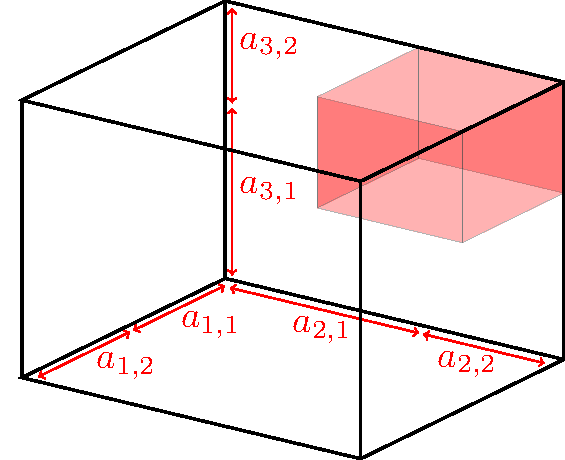
\includegraphics[width=0.4\textwidth]{figures/2/recursion.pdf}
\caption{A recursively constructed $[b_1] \times [b_2] \times [b_3]$ grid, for $n = 2$, $d = 3$.}
\label{fig:recursion}
\end{figure} 

\begin{lem}
\label{lem:recursion}
For $n,d \geq 1$, let $A = (a_{i,j})$ be a $d \times n$ matrix of positive integers, and let $b_i = \sum_{j=1}^n a_{i,j}$, for $1 \geq j \geq d$. Let $S$ be a lethal set under the modified process on $[n]^d$, and for each vertex $\vec{x} = (x_1, \dots, x_v) \in S$, let $T_{\vec{x}}$ be a lethal set on $\prod_{i=1}^d [a_{i,x_i}]$ under $d$-neighbor percolation. Then
$$m(b_1, \dots, b_d, d) \leq \sum_{\vec{x} \in S} |T_{\vec{x}}|.$$
\end{lem}

\begin{proof}
We imagine sub-dividing the $\prod_{i=1}^d [b_{i}]$ brick into smaller blocks by partitioning each of the $d$ axes into segments $a_{i,1}, a_{i,2}, \dots, a_{i,n}$, $1 \leq 1 \leq d$. 
\end{proof}

% Handle the divisibility cases, and note that certain augmentations to the recursion allow us to obtain non-divisible optimal grids, if we are cautious with regard to the pieces we use.

\section{Examples and Notation}

% Discuss that the recursion works by assembling any set of compatible n^2 blocks, although it is very rare that it is necessary to use more than 4. 
% Talk about the component pieces necessary to assemble a brick of size (a,b,c).

% Should we talk about the broad behavior of percolating sets?
\section{Regional vs. Temporal Infections}

